\documentclass[12pt,a4paper, spanish]{report}
\usepackage[spanish]{babel}
\usepackage[latin1]{inputenc}  % Ambos para solucin de asuntos de idioma
\usepackage[T1]{fontenc}
\usepackage{tocbibind}  % Bibliografa en el indice
\usepackage{titlesec}  % Posibilidad de editar los formatos de chapter y section
%\usepackage{times}  % Fuente de letras
\usepackage{amsmath,amssymb,mathrsfs,mathptmx}  % Matemticas varias
\usepackage{hyperref} % Para escribir URLs



% --- Arreglos varios para la inclusion de imgenes
%\usepackage[pdftex]{graphicx}
%\usepackage[dvips]{graphicx}
\usepackage{graphicx}
\usepackage{epstopdf}
\usepackage{float}
\usepackage{subfigure}
%\usepackage{subfig}
\usepackage{wrapfig}
\usepackage[usenames,dvipsnames]{color}
\DeclareGraphicsExtensions{.png,.jpg,.pdf,.mps,.gif,.bmp, .eps}


	

\usepackage{multirow}
\usepackage{multicol}
\usepackage{tabulary}
\usepackage[table]{xcolor}
\usepackage{color}
\usepackage{listings}
%\usepackage{subfloat}
\usepackage{tikz}

\setcounter{secnumdepth}{3}
\setcounter{tocdepth}{3}


% --- Para las dimensiones de los mrgenes etc
\frenchspacing \addtolength{\hoffset}{-1.5cm}
\addtolength{\textwidth}{3cm} \addtolength{\voffset}{-2.5cm}
\addtolength{\textheight}{4cm}
% --- Para el encabezado
\usepackage{fancyhdr}
\fancyhead[R]{2012}\fancyhead[L]{enCuadro} \fancyfoot[C]{\thepage}
\pagestyle{fancy}

% --- Formato de la etiqueta Chapter
%\newcommand{\bigrule}{\titlerule[0.5mm]}
%\titleformat{\chapter}[display]{\bfseries\Huge}
%{\Large\chaptertitlename\ \Large\thechapter}
%{0mm} {\filleft} [\vspace{0.5mm} \bigrule]

\titleformat{\chapter}[display]
{\normalfont\Large\filcenter}
{\titlerule[1pt]%
\vspace{1pt}%
\titlerule
\vspace{1pc}%
\LARGE\MakeUppercase{\chaptertitlename} \thechapter}
{1pc}
{\titlerule
\vspace{1pc}%
\Huge}

%-------------------------

\begin{document}
% Esto es para que se muestren todas las referencias aunque no se citen:
\nocite{*}

\renewcommand{\tablename}{Tabla}
\renewcommand{\theenumi}{\Roman{enumi}}
\renewcommand{\labelenumi}{[\textbf{\theenumi}]}
\renewcommand{\thefootnote}{\arabic{footnote}}
% --- Modificacin de entornos enumerate
\renewcommand{\theenumi}{\roman{enumi}}
\renewcommand{\labelenumi}{\theenumi)}
% --- Modificacin de entornos enumerate

% --- Para hacer highlights
\newcommand{\highlAmarillo}[1]{\colorbox{yellow}{#1}}
\newcommand{\highlVerde}[1]{\colorbox{green}{#1}}
\newcommand{\highlRojo}[1]{\colorbox{red}{#1}}

%



\chapter{Identificaci�n}
\label{chap: ident}
\section{Introducci�n}
Introducci�n
\section{T�cnicas de identificaci�n}
T�cnicas de identificaci�n


\section{QR}
Ventajas del Lenguaje C para procesamiento de im�genes

\subsection{Identificadores QR: una realidad cotidiana.}
El uso de los identificadores QR (Quick Response), es cada vez m�s generalizado. �ltimamente, debido al incremento significativo del uso de \textit{smart devices}, el hecho de poder contar con una c�mara, cierto poder de procesamiento y por lo general hasta una conexi�n m�vil a internet, hace que sea cada vez m�s frecuente encontrar aplicaciones con el poder de reconocer QRs. Comenzaron utiliz�ndose en la industria automovol�stica japonesa como una soluci�n para el trazado en la l�nea de producci�n, pero su campo de aplicaci�n se ha diversificado y hoy en d�a se pueden encontrar tambi�n como identificatorios de entradas deportivas, tickets de avi�n, localizaci�n geogr�fica, v�nculos a p�ginas web y en algunos casos tambi�n como tarjetas personales. 
\subsection{?`Qu� son los QR?}
Los QRs son una extensi�n de los c�digos de barras. Incorporan una segunda dimensi�n lo cual es una gran ventaja ya que pueden almacenar mucho m�s informaci�n. Existen distintos tipos de QR, con distintas capacidades de almacenamiento que dependen de la versi�n, el tipo de datos almacenados y del tipo de correcci�n de errores. En su versi�n 40 con detecci�n de errores de nivel L, se pueden almacenar alrededor de 4300 caracteres alfanum�ricos o 7000 d�gitos (frente a los 20-30 d�gitos del c�digo de barras) lo cual lo hace muy flexible para cualquier tipo de aplicaci�n de identificaci�n.\\

En la Figura \ref{fig: implementacion_2} se pueden ver las distintas partes que componen un QR, como por ejemplo el bloque de control, compuesto por las tres esquinas id�nticas que dan informaci�n de la posici�n, la informaci�n de alineamiento y el patr�n de sincronismo; as� como tambi�n la indicaci�n de versi�n, formato y la correcci�n de errores. Fuera de toda esa informaci�n, que podr�a verse como el encabezado, haciendo analog�a con los paquetes de las redes de datos, se encuentran los datos propiamente dicho, que podr�an verse como el cuerpo del paquete.\\
\begin{figure}[h!]
\centering
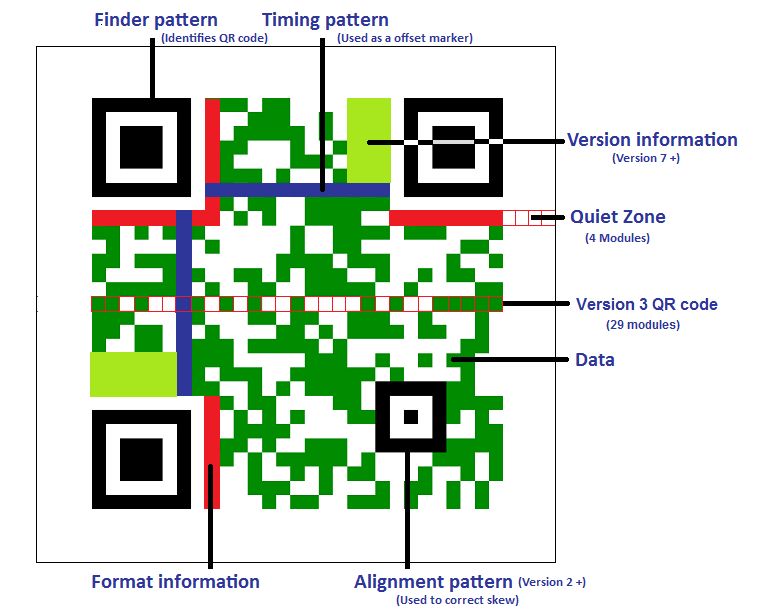
\includegraphics[scale=0.4]{figs_identificacion/qrcode_overview4.png}
\caption{Las distintas componentes de un QR. Fuente (poner fuente).}
\label{fig: implementacion_2}
\end{figure}
%fuente http://www.qrme.co.uk/qr-code-resources/understanding-a-qr-code.html


\subsection{Codificaci�n y decodificaci�n de c\'odigos QR.}

Es f�cil darse cuenta que la codificaci�n resulta mucho m�s sencilla que la decodificaci�n. Para la codificaci�n es necesario comprender el protocolo, las distintas variantes y el tipo de informaci�n que se pretende almacenar. Sin embargo, para la decodificaci�n, adem�s de tener que cumplir con lo anterior, es necesario contar con buenos sensores y ciertas condiciones de luminosidad y distancia que favorezcan a la c�mara y se traduzcan en buenos resultados luego de la detecci�n de errores. Si bien la plataforma es importante para lograr buenos resultados, dada una plataforma, existen variadas aplicaciones tanto para iOS como para Android que cuentan con performances bastante diferentes en funci�n del algoritmo de procesamiento utilizado.\\

Debido a que el centro del presente proyecto no fue la codificaci�n y decodificaci�n de QRs, y que adem�s ya existen distintas librer�as que resuelven muy bien este problema, se opt� por investigar varias de ellas e incorporar la m�s adecuada a la aplicaci�n.\\

Entre todas las librer�as que resuelven la decodificaci�n, las llamadas ZXing y ZBar son quiz� las m�s destacadas, por su popularidad, simplicidad y buena documentaci�n para la f�cil implementaci�n. ZXing, denominada as� por ``Zebra Crossin'', es una librer�a gratis y en c�digo abierto desarrollada en java y que tiene implementaciones que est�n adaptadas para otros lenguajes como C++, Objetive-C y JRuby, entre otros.\\

Por su parte ZBar tambi�n tiene soporte sobre varios lenguajes y cuenta con un kit de desarrollo interesante para lograr f�cilmente aplicaciones que integren el lector de QR. Se trabaj� sobre el c�digo de ejemplo que contiene la implementaci�n de las clases principales para obtener un lector y finalmente se opt� por utilizar esta librer�a para los fines de la aplicaci�n. El lector del c�digo de ejemplo consta de una clase \textit{ReaderSampleViewController} que hereda de \textit{UIViewController} y que implementa un protocolo llamado \textit{ZBarReaderDelegate}. Al presionarse el bot�n de detecci�n se crea una instancia de la clase \textit{ReaderSampleViewController} y se presenta la vista previa de la c�mara. Luego el protocolo se encarga de la captura y procesamiento del QR almacenando como resultado la informaci�n embebida en este en la variable denominada \textit{ZBarReaderControllerResults}. Esta variable luego se mapea en una \textit{hash table} con el contenido en formato \textit{NSDictionary}. De esta manera se accede f�cilmente al contenido en formato legible y es f�cil de hacer una l�gica de comparaci�n y b�squeda en una base de datos.\\
%fuente http://code.google.com/p/zxing/


\subsection{Expresiones art�sticas con QRs.}
La opci�n de usar los QR de una manera distinta ha comenzado a ser notoria en los �ltimos tiempos. Hay quienes desaf�an a la informaci�n \textit{cruda de 1s y 0s} incorporando im�genes y modificando colores y contornos en los QR tradicionales para lograr un valor est�tico adem�s del funcional. V\'ease en la Figura \ref{fig: implementacion_3} un ejemplo de c�mo puede lograrse el mismo resultado pero con el valor agregado de originalidad.

\begin{figure}[h!]
\centering

\includegraphics[scale=0.2]{figs_identificacion/qrArtist.png}
\caption{Ejemplo de un QR creativo. Fuente (poner fuente).}
\label{fig: implementacion_3}
\end{figure}
%fuente http://www.qrcartist.com/wordpress/wp-content/uploads/2012/10/studiothirt3-gr.png


\section{SIFT}
\label{sec: sift}
El algoritmo SIFT, acr\'onimo de ``Scale Invariant Feature Transform'',  es un algoritmo de visi\'on artificial \cite{Lowe:2004}, \cite{Lowe:1999}, que se encarga de extraer caracter\'isticas distintivas de las im\'agenes en escala de grises. Mediante estas, es posible luego reconocer dicha imagen dentro de una base de datos o incluso dentro de otra imagen mayor con otra cantidad de elementos en desorden. Estas caracter\'isticas son invariantes a factores de escala, traslaci\'on, rotaci\'on y parcialmente invariantes a cambios de iluminaci\'on y afinidades. El algoritmo consta b\'asicamente de cuatro pasos que se explicar\'an brevemente en secciones subsiguientes.\\ 

\subsection{Detecci\'on de extremos en el espacio-escala.}
Se busca encontrar dentro del \textit{scale-space} (espacio-escala) de la imagen puntos caracter\'isticos; invariantes a la traslaci\'on, el escalado y la rotaci\'on de la misma. Adem\'as esos puntos deben ser m\'inimamente afectados por el ruido y peque\~nas distorsiones. Ser\'an los puntos extremos (m\'aximos o m\'inimos) obtenidos de las diferencias Gaussianas aplicadas al \textit{scale-space} de la imagen. El \textit{scale-space} de una imagen se define como una familia de im\'agenes $L(x,y,\sigma)$ que se obtienen de convolucionar un n\'ucleo Gaussiano variable en su desviaci\'on est\'andar $G(x,y,\sigma)$ con una imagen de entrada $I(x,y)$:
\[
L(x,y,\sigma) =  G(x,y,\sigma) * I(x,y)
\]
donde $*$ denota la convoluci\'on en $x$ e $y$, y adem\'as:
\[
G(x,y,\sigma) = \frac{1}{2\pi{\sigma}^2}{\rm e}^{-\frac{x^2 + y^2}{2\sigma^2}} 
\]

Una imagen diferencia de Gaussianas, $D(x,y,\sigma)$, se define entonoces de la siguiente manera:\\
\[
D(x,y,\sigma) = L(x,y,k\sigma) - L(x,y,\sigma) 
\]
con $k$ un factor multiplicativo constante.\\

Dado un valor inicial para $\sigma$, se le realiza a la imagen un n\'umero $s$ de diferencias Gaussianas con la desviaci\'on est\'andar variando de manera creciente a lo largo de una octava (hasta obtener un $\sigma' = 2\sigma$). Para obtener $s$ intervalos enteros dentro de dicha octava el valor de $k$ en cada diferencia Gaussiana debe ser de $2^{\frac{1}{s}}$. Una vez calculadas las diferencias Gaussianas a lo largo de la octava, la imagen se submuestrea tomando 1 de cada 2 p\'ixeles en filas y columnas y se procede de la misma manera. La cantidad de octavas involucradas en el c\'alculo as� como la cantidad de diferencias Gaussianas calculadas por octava son un par\'ametro a determinar. En la Figura \ref{fig:SIFT_1} se puede ver lo anterior explicado gr\'aficamente.\\
\begin{figure}[h!]
\centering
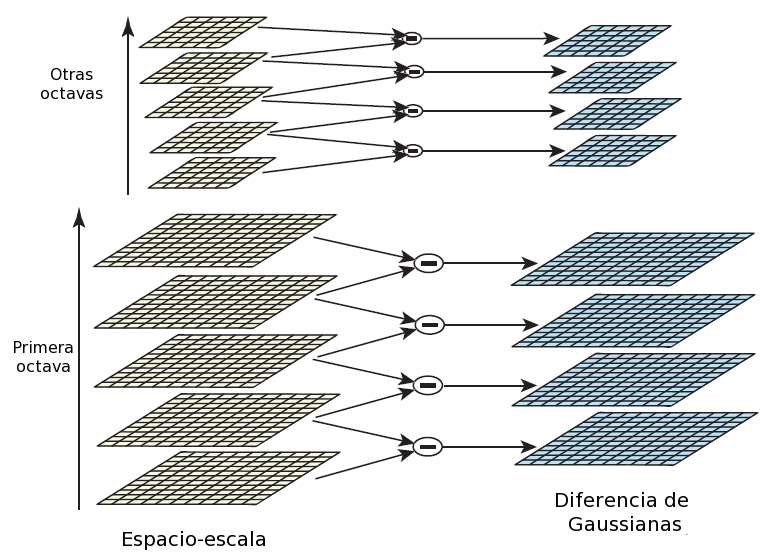
\includegraphics[scale=0.4]{figs_identificacion/SIFT_1.png}
\caption{Para cada octava, la imagen original es convolucionada repetidamente con Gaussianas de desviaci\'on est\'andar variable para producir el \textit{scale-space} de la izquierda. Im�genes adyacentes del \textit{space-scale} son restadas para lograr la diferencia de Gaussianas de la derecha. Despu\'es de cada octava, la imagen borrosa es submuestreada por un factor de dos y el proceso se repite. Figura tomada de \cite{Lowe:2004}.}
\label{fig:SIFT_1}
\end{figure}

Una vez que se obtiene la ``pir\'amide'' de diferencia de Gaussianas anterior, se buscan para cada ``piso'' de la misma extremos locales quienes se transformar\'an en candidatos a puntos clave. Para una $D(x,y,\sigma)$ determinada y en una octava determinada, un punto $(x_0,y_0)$ ser\'a un m\'aximo (m\'inimo) relativo si es mayor (menor) a sus 8 puntos vecinos dentro de su nivel y a sus 9 puntos vecinos de cada uno de los niveles inferior y superior. Si el punto se encuentra en una $D(x,y,\sigma)$ de transicion entre 2 octavas, se buscan los puntos vecinos correspondientes del nivel superior (inferior). Ver Figura \ref{fig:SIFT_2}. \\

\begin{figure}[h!]
\centering
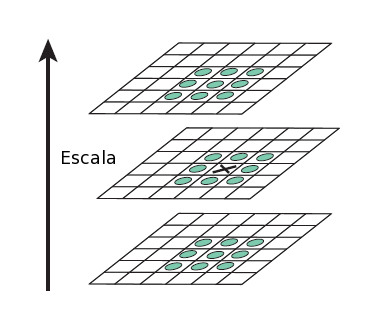
\includegraphics[scale=0.4]{figs_identificacion/SIFT_2.png}
\caption{M\'aximos y m\'inimos de las im\'agenes diferencia de Gaussianas son obtenidos comparando cada p\'ixeles con sus vecinos en la misma escala, y en las escalas adyacentes. Figura tomada de \cite{Lowe:2004}.}
\label{fig:SIFT_2}
\end{figure}
% -------------------------------------------------------------------------------------------------------------------------------------------

\subsection{Localizaci\'on exacta de puntos clave.}
La b\'usqueda de extremos en las diferencias de Gaussianas produce m\'ultilpes candidatos entre los que se encuentran puntos con poco contraste;  los cuales no son estables a cambios de iluminaci\'on y al ruido. Para quitarlos se procede de la siguente manera.\\

Primero se realiza una expansi\'on de Taylor de grado 2 entorno a cada extremo detectado $(x_0,y_0,\sigma_0)$:
\begin{equation}
D(\chi) = D + \frac{\partial D^T}{\partial \chi} \chi + \frac{1}{2}{\chi}^T\frac{\partial^2D}{\partial {\chi}^2} \chi
\label{eq:1}
\end{equation}
donde $D$ y sus derivadas son evaluadas siempre en el punto en cuesti\'on y $\chi = (x,y,\sigma)^T$ es la posici\'on relativa al mismo. Derivando la aproximaci\'on anterior e igual\'andola a cero se obtiene:\\
\begin{equation}
\bar{\chi} = -\frac{\partial ^2D^{-1}}{\partial {\chi^2}}\frac{\partial D}{\partial \chi}
\label{eq:2}
\end{equation}
Reemplazando (\ref{eq:2}) en (\ref{eq:1}) se obtiene el valor del m\'aximo local:\\
\[
D(\bar{\chi}) = D + \frac{1}{2}\frac{\partial D^T}{\partial \chi} \bar{\chi}
\]
Finalmente, si $\left| D(\bar{\chi}) \right|< 0.03$ el punto es eliminado de la lista de puntos clave; suponiendo que D toma valores entre 0 y 1.\\

Adem\'as de quitar aquellos puntos con poco contraste, hay que quitar a los puntos candidatos que pertenecen a una l\'inea y no a una esquina. Para ello, sea $H$ la matriz Hessiana de $D(x,y,\sigma)$ evaluada en un punto extremo de las diferencias de Gaussianas determinado $(x_0,y_0,\sigma_0)$, se estar\'a en presencia de un borde (l\'inea) si sus valores propios $\alpha$ y $\beta$ son uno grande y el otro peque\~no. Lo anterior es equivalente a trabajar con los siguientes resultados:\\
\[
Traza(H) = \frac{\partial^2 D}{\partial x^2} + \frac{\partial^2 D}{\partial y^2} = \alpha +\beta
\]
\[
Det(H) = \frac{\partial^2 D}{\partial x^2} \times \frac{\partial^2 D}{\partial y^2} - \left(\frac{\partial^2 D}{\partial x. \partial y} \right)^2= \alpha . \beta
\]
Sea la $\alpha = r.\beta$, la condici\'on se reduce a:\\
\[
\frac{Traza(H)^2}{Det(H)} < \frac{(r+1)^2}{r}
\]
Luego de varios experimentos, se propone un umbral de $r=10$. V\'ease que conforme aumenta la relaci\'on $r$ entre ambos valores propios tambi\'en lo hace la relaci\'on entre el cuadrado de la traza de la matriz Hessiana y su determinante.\\

% -------------------------------------------------------------------------------------------------------------------------------------------
\subsection{Asignaci\'on de orientaci\'on.}
Mediante la asignaci\'on de una orientaci\'on a cada punto de la imagen basada en caracter\'isticas locales de la misma, los puntos clave pueden ser descriptos relativos a estas orientaciones y de esta manera lograr caracter\'isticas invariantes a las rotaciones. Para cada punto clave obtenido $D (x_0,y_0,\sigma_0)$ , se busca su imagen borrosa correspondiente en el espacio escala $L (x,y,\sigma_0)$ y se determina el m\'odulo de su gradiente $m(x,y)$ y la fase del mismo $\theta (x,y)$ utilizando diferencias entre p\'ixeles:\\
\[
\begin{array}{c}
m(x,y) = \sqrt{ (\Delta L_x)^2 + (\Delta L_y)^2} \\ 
m(x,y) = \sqrt{[L(x+1,y) - L(x-1,y)]^2 + [L(x,y+1) - L(x,y-1)]^2}
\end{array}
\]
\[
\begin{array}{c}
\theta(x,y) = tan^{-1}\left( \frac{\Delta L_y}{\Delta L_x}\right) \\ 
\theta(x,y) = tan^{-1}\left( \frac{L(x,y+1) - L(x,y-1)}{L(x+1,y) - L(x-1,y)}\right) 
\end{array}
\]

Para determinar de una forma fiel la orientaci\'on de cada punto clave, \'esta es determinada tomando en cuenta las direcciones de todos los puntos de la imagen dentro de cierto entorno al mismo. Se genera entonces un histograma de direcciones con valores que var\'ian de a 10 grados, ponderado por el m\'odulo del gradiente y una ventana Gaussiana circular centrada en el punto clave, de desviaci\'on est\'andar igual a 1.5 veces el valor del nivel del en cuesti\'on. Cada m\'aximo en el histograma corresponde a la direcci\'on dominante en el gradiente local y ser\'a la asignada al punto clave. Si existen en el histograma otros m\'aximos secundarios de valor mayor o igual al $80\%$ del m\'aximo principal, estos ser\'an utilizados para generar nuevos puntos clave con esa direcci\'on. S\'olo al $15\%$ de los puntos clave se les asigna m\'as de una direcci\'on.\\
% -------------------------------------------------------------------------------------------------------------------------------------------
\subsection{Descriptor de puntos clave.}
\begin{figure}[h!]
\centering
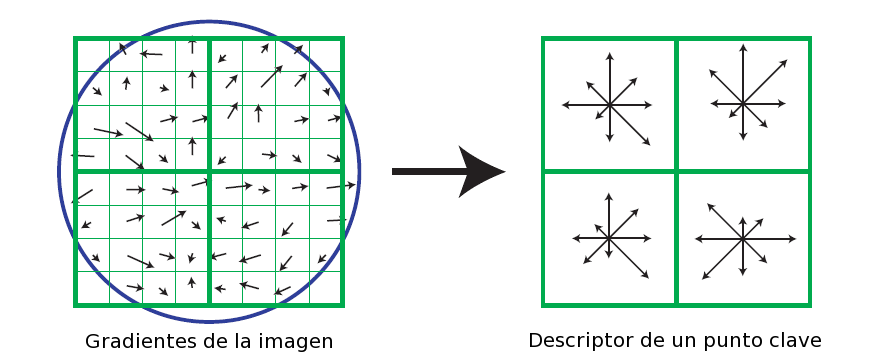
\includegraphics[scale=0.4]{figs_identificacion/SIFT_3.png}
\caption{Izq.: La ventana Gaussiana pondera los valores de m\'odulo y fase en la vecindad de los puntos de inter\'es. Der.: los histogramas con 8 direcciones posibles realizados para cada subregi\'on. Figura tomada de \cite{Lowe:2004}.}
\label{fig:SIFT_3}
\end{figure}

Hasta el momento, se le ha asignado a cada punto clave una escala, una locaci\'on y una orientaci\'on. El siguiente paso es determinar para cada punto clave un descriptor relativamente invariante a cambios de iluminaci\'on y afinidades, basado en el entorno del mismo.\\

Una vez determinadas la magnitud y fase del gradiente entorno a un punto clave, una ventana Gaussiana centrada en este pondera los valores de m\'odulo y fase de $4\times 4$ subregiones cuadradas en la vecindad del mismo, cada una formada por $16$ p\'ixeles. Nuevamente se genera para cada subregi\'on un histograma de 8 direcciones distintas. Se obtiene finalmente para cada punto clave un descriptor de $4\times 4 \times 8 = 128$ valores.\\

En la Figura \ref{fig:SIFT_3} se ve c\'omo se computan los descriptores para cada punto clave. En el ejemplo se utilizan \'unicamente $2\times 2 = 4$ subregiones en vez de $4\times 4 = 16$.\\


% Ejemplo de como hacer una cita:
\cite{Daniel03simultaneouspose}.



\bibliographystyle{unsrt}   
\bibliography{encuadro}  
\end{document}
